Die grundlegende Programmierausbildung im Department Informatik an der HAW Hamburg erfolgt in der Programmiersprache Java, weswegen auch die Funktionen von Weclare auf Java ausgerichtet sind. Normalerweise wird Java in einem zweistufigen Prozess ausgeführt. Zunächst wird eine plattformabhängige Java Virtual Machine (JVM) geladen. Innerhalb dieser JVM wird der Java-Compiler (javac) aufgerufen. Dieser compiliert Java-Quelltext zu Java-Bytecode. Der Java-Bytecode kann dann von der JVM ausgeführt werden. Dieser Ablauf ist in der Abbildung \ref{abb:java_execution} unter a) dargestellt.

Um Java in einem Browser auszuführen ergeben sich konzeptionell mindestens drei verschiedene Möglichkeiten, die in Abbildung \ref{abb:java_execution} mit den Buchstaben b - d gekennzeichnet sind.

\begin{figure}[H]
    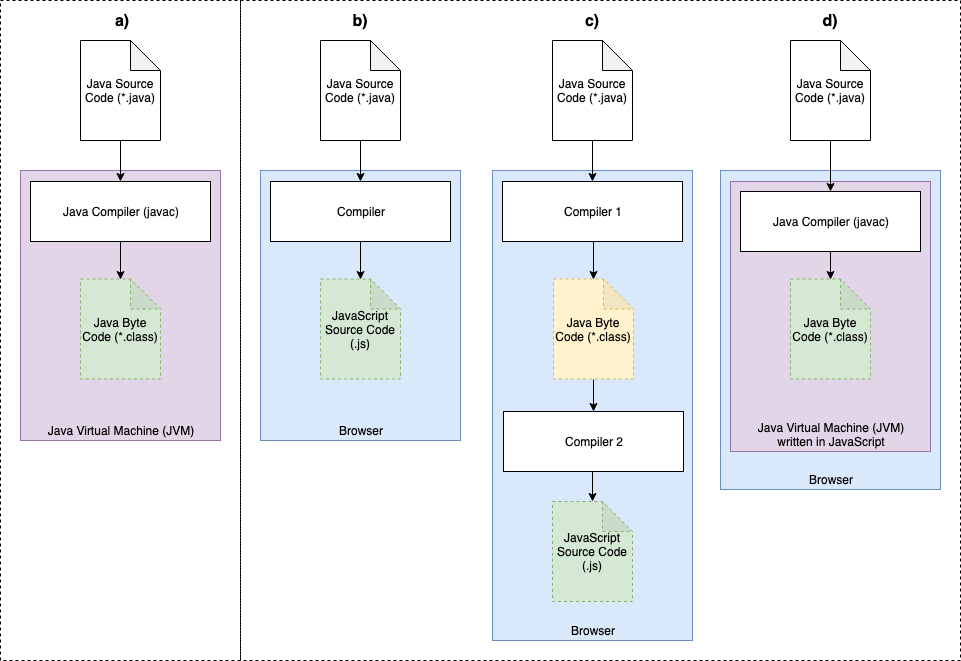
\includegraphics[width=14cm]{chapter/entwurf/bilder/Java_JavaScript_Execution.png}
    \centering
    \caption{Blubb}
    \label{abb:java_execution}
\end{figure}

\begin{itemize}
    \item \textbf{b:} Java-Quelltext wird mit einem Compiler direkt in JavaScript umgewandelt: Diese Variante ist konzeptionell sehr einfach. Zwar gibt es einige Programme, welche Java-Quelltext in JavaScript übersetzen können (zum Beispiel JSweet oder GWT), jedoch sind alle diese Programme entweder in Java selbst oder in dritten Programmiersprachen verfasst. Einen solchen Compiler, der selbst in JavaScript geschrieben wurde und damit auch im Browser ausgeführt werden kann gibt es wohl nicht. Es wäre möglich eines der besagten Programme auf einem separaten Server einzusetzen. Dies würde aber eine weitere Abhängigkeit von einem Server bedeuten, und damit den formulierten Kern-Anforderungen widersprechen.
    \item \textbf{c:} Java-Quelltext wird mithilfe eines ersten Compilers in Java-Bytecode übersetzt. Anschließend wird der Java-Bytecode mit einem zweiten Compiler in JavaScript übersetzt. Auch hier ergibt sich das gleiche Problem wie in b). Zwar gibt es Programme, die den jeweiligen Teilschritt übernehmen könnten, jedoch ist keins davon in JavaScript verfasst, so dass es keine browserkompatible Lösung dafür gibt.
    \item \textbf{d:} Wie auf einem lokalen Rechner wird eine JVM zur Ausführung verwendet, die allerdings selbst in JavaScript implementiert wurde. Mithilfe dieser JVM können existierende Java-Programme wie zum Beispiel der javac-Compiler ausgeführt werden, um Java-Quelltext in Java-Bytecode zu übersetzen und das Ergebnis kann anschließend ausgeführt werden.
\end{itemize}

In Anbetracht der Tatsache, dass die Ausführung der Code-Beispiele im Browser exakt die gleichen Ergebnisse liefern soll, wie die Ausführung in einer lokalen JVM (zum Beispiel auch in Bezug auf Fehler beim Kompilieren), so ist die Variante d die bevorzugte Lösung und wird im Rahmen dieser Arbeit in das entstandene CRS integriert.

Die benötigte JVM-Implementierung in JavaScript existiert bereits in Form eines Universitätsprojekts der PLASMA-Forschungsgruppe der University of Massachusetts in Amherst, USA. Unter dem Namen DoppioJVM wurde dort im Jahr 2014 im Rahmen einer wissenschaftlichen Arbeit eine solche JVM erschaffen:

\begin{quotation}
„DoppioJVM is a robust prototype Java Virtual Machine (JVM) interpreter
that operates entirely in JavaScript. DoppioJVM implements all 201 bytecode instructions specified in the second edition of the Java Virtual Machine Specification, supports multithreaded programs, runs multiple languages that run on top of the JVM, and implements many of the complex mechanisms and native functionality that JVM programs expect.“
\end{quotation}

Voraussetzung für die Nutzung von DoppioJVM ist ein weiteres Projekt der gleichen Forschungsgruppe namens BrowserFS. Die JVM benötigt Zugriff auf ein Dateisystem, welches der Browser als Laufzeitumgebung normalerweise nicht anbietet. Wer JavaScript außerhalb des Browser auf dem Server bzw. in der Kommandozeile einsetzt kann aber dank der Node.js-Laufzeitumgebung auf Dateisysteme zugreifen. Genau diese populäre Node.js-API emuliert BrowserFS und bringt sie in den Browser. Dabei werden verschiedene Datenquellen unterstützt: Die Dateien können zum Beispiel im LocalStorage des Browser oder aber komplett im Arbeitsspeicher abgelegt werden. Für den Betrieb der DoppioJVM zum Beispiel werden zwei Verzeichnisse mit verschiedenen Datenquellen installiert: Die Bestandteile der JRE werden auf dem Webserver abgelegt und anschließend beim Zugriff über asynchrone HTTP-Requests nachgeladen (AJAX). Die Quelltext- und Bytecode-Dateien, mit denen die JVM arbeitet, werden komplett im Arbeitsspeicher abgelegt.

Nachdem das BrowserFS-Dateisystem konfiguriert ist, kann DoppioJVM mit einer relativ einfachen Schnittstelle verwendet werden:

\begin{minipage}{\linewidth}
\begin{lstlisting}[caption={Instantiierung der DoppioJVM (aus: src/server/actions/doppio.js)}]
new Doppio.VM.JVM(
  {
    doppioHomePath: "/sys",
    classpath: [".", "/sys/", "/tmp/"]
  },
  (err, jvmObject) => {
    jvmObject.runClass("Loader", [classname], exitCode => {
      if (exitCode !== 0) {
        console.log("JVM exited with an error");
      } else {
        console.log("JVM exited successfully");
      }
    });
  }
);
\end{lstlisting}
\end{minipage}

Die DoppioJVM muss bei jeder Verwendung neu instantiiert werden. Deswegen ist es erforderlich, dass die Kompilierung und Ausführung des gewünschten Java-Codes in einem Aufruf erfolgt. Dazu bietet Java zum Glück die passenden Klassen und Methoden um Quelltexte programmatisch zu kompilieren und auszuführen:

\begin{minipage}{\linewidth}
\begin{lstlisting}[caption={Java-Loader, der programmatisch Quelltext kompiliert und ausführt. (aus: public/doppio/Loader.java)}]
import javax.tools.*;
import java.lang.reflect.*;
import java.io.*;
import java.net.*;

public class Loader {
  public static void main(String[] args) {
    if (args.length == 0) {
      System.out.println("No class was found.");
      System.exit(1);
    }
    String className = args[0];
    String sourceFile = "/tmp/" + className + ".java";
    String classFile = "/tmp/" + className + ".class";

    System.out.println("Compiling found class '" + className + "'...");

    JavaCompiler compiler = ToolProvider.getSystemJavaCompiler();
    int result = compiler.run(null, null, null, sourceFile, "-d", "/tmp/");

    if (result == 0) {
      try {
        System.out.println("Compilation successful. Executing...");
        System.out.println("---");

        URLClassLoader classLoader = new URLClassLoader(
            new URL[] {new File(classFile).toURI().toURL()}, ClassLoader.getSystemClassLoader());
        Class<?> c = classLoader.loadClass(className);
        Method m = c.getDeclaredMethod("main", String[].class);
        m.invoke(null, new Object[] {});
        classLoader.close();

        System.out.println("Execution successfull");
      } catch (Exception e) {
        e.printStackTrace();
      }
    } else {
      System.out.println("Could not compile");
    }
  }
}
\end{lstlisting}
\end{minipage}

Ebenso wie die Netzwerk-Kommunikation ist auch die Instanziierung der DoppioJVM in Form von ActionCreator-Funktion in Weclare integriert um dem Flux-Muster zu entsprechen. In einem Store wird dabei auch der Inhalt des kleinen Terminal-Fensters gespeichert, welches die Standard-Streams der DoppioJVM abfängt.

\begin{figure}[H]
    \centering
    \setlength{\fboxsep}{0pt}
    \setlength{\fboxrule}{0.5pt}
    \fbox{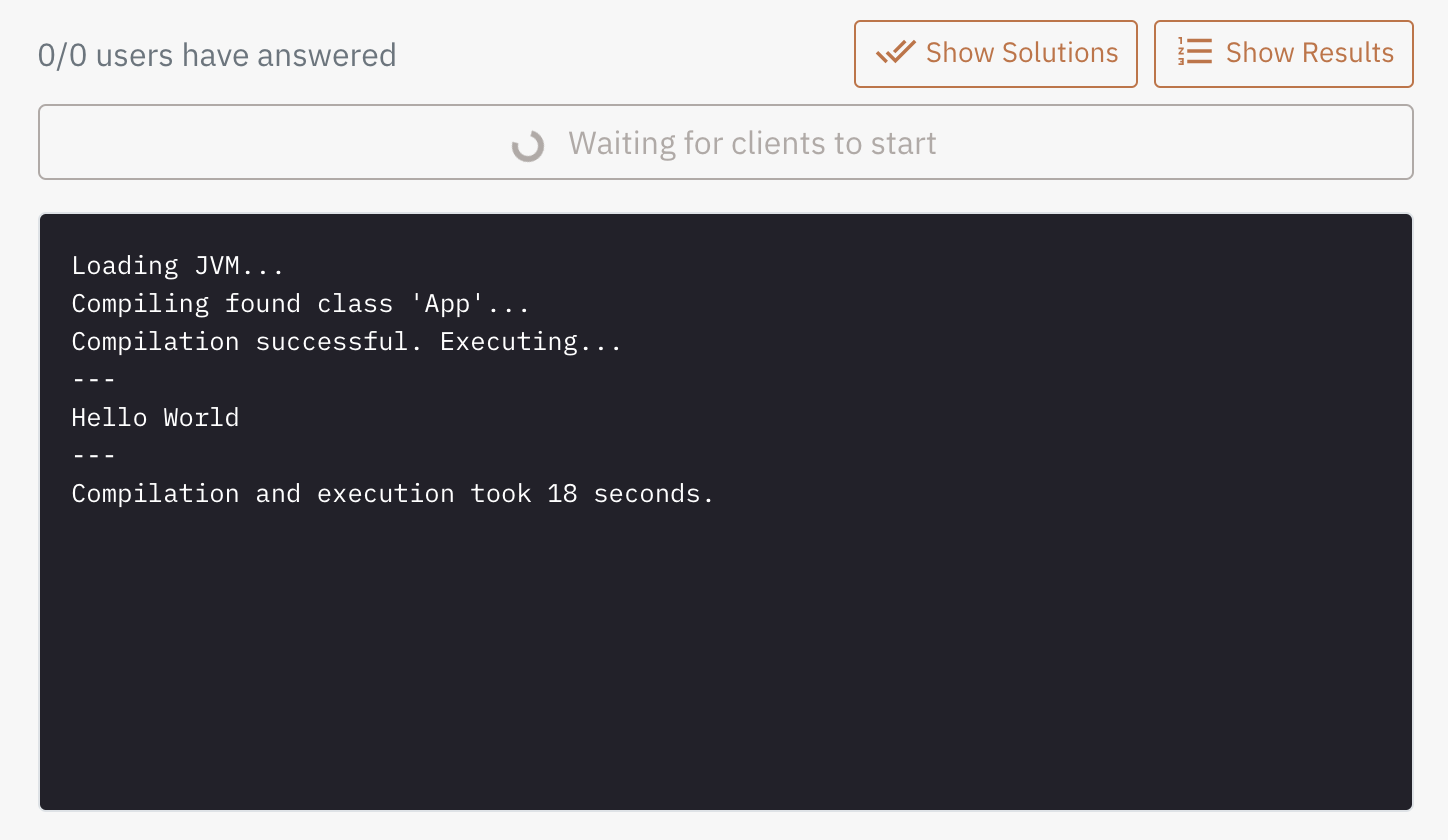
\includegraphics[width=\textwidth-1pt]{chapter/entwurf/bilder/weclare_jvm_console.png}}
    \caption{Ausführung einer Java-Klasse in Weclare mittels DoppioJVM.}
    \label{abb:weclare_jvm_console}
\end{figure}

